\section{Background}

\subsection{Required Notation}

We first define some pertinent notation used in this paper.
A random variables is denoted by upper-case letter $X$.
The values of $X$ are denoted by $val(x)$, where lower-case element $x$ is a corresponding element of $val(X)$.
Sets of random variables are defined by boldface letter ${\bf X}$.
For ${\bf X} = \{X_1,\dots,X_N\}$, we define ${\bf val(X)} = \times^{N}_{n=1}{{\bf val}(X_n)}$ and use corresponding lower-case boldface  letters for elements of ${\bf val(X)}$.
For a subset ${\bf Y \subseteq X}$, ${\bf x[Y]}$ is a projection of ${\bf x}$ onto ${\bf Y}$.

Let ${\cal G}$ denote a \emph{directed acyclic graph} (DAG) on a finite set of variables (nodes).
A \emph{directed path} from $v_1$ to $v_k$ is a sequence $v_1, v_2, \ldots , v_k$ with directed edges $(v_i, v_{i+1})$ in ${\cal B}$, $i = 1, 2,\ldots, k-1$.
For each $v_i \in U$, the \emph{ancestors} of $v_i$, denoted $An(v_i)$, are those variables having a directed path to $v_i$.
For a set $X \subseteq U$, we define $An(X)$ in the obvious way.
The \emph{children} $Ch(v_i)$ and \emph{parents} $Pa(v_i)$ of $v_i$ are those $v_j$ such that $(v_i,v_j) \in {\cal G}$ and $(v_j,v_i) \in {\cal G}$, respectively.
%A singleton set $\{v\}$ may be written as $v$ and $\{ v_1, v_2, \ldots, v_n \}$ as $v_1 v_2 \cdots v_n$.
The cardinality of a set $W$ is denoted $|W|$.


\subsection{Sum-Product Networks}

A \emph{Sum-Product network} (SPN) $\cal S$ over Boolean variables ${\bf X} = \{X_1,\dots,X_N\}$ is a rooted DAG which contains three types of nodes: indicators, sums and products.
All leaves of $\cal S$ are indicator variables $\lambda_{x_1},\ldots,\lambda_{x_N}$ and $\lambda_{\bar{x}_1},\ldots,\lambda_{\bar{x}_N}$.
All internal nodes are either sum or product.
An indicator variable $\lambda[X=x]$ returns 1 when $X=x$ and 0 otherwise.
Each edge $(v_i,v_j)$ from a sum node $v_i$ has a non-negative weight $w_{ij}$.
The value of a product node is the product of its children.
The value of a sum node is $\sum_{v_j \in Ch{v_i}}{w_{ij}val(v_j)}$.

%
%For $x \in {\bf val(X)}$, we define indicator variables $\lambda_{X=x}(x) := 1(x =x^\prime)$ as input distribution.
%
%graph together with non-negative weights $w_{ij}$ for each edge $(w_i,w_j)$. 

% random variable $X$ with finitely states 
Figure \ref{fig:spn} shows an SPN over random variables variables ${\bf X}=\{X_1,X_2,X_3\}$.
[Say that for simplicity, as for Poupart, we are using Boolean variables.]
An SPN can be extended for multi-valued discrete variables by replacing Boolean indicators for the variables's possible values.
For instance, a multinomial distribution over $X_i$ can be represented by $\sum_{j=1}^{m}{p^j_i x^j_i}$, where $p^j_i = P(X_i = x^j_i)$.


\begin{figure}[h]
    \begin{center}
		\includegraphics[width=0.5\textwidth]{figures/SPN.png}
		\caption{Example SPN from over ${\bf X}=\{X_1,X_2,X_3\}$ adapted from \cite{Peharz:2016wl}.}
		\label{fig:spn}
    \label{fig:spn}
    \end{center}
\end{figure}

\begin{example}
Show example with $P(E=e)$ and indicator variables.	
\end{example}

The \emph{scope} of a node $v$ in an SPN $S$ is defined as
\begin{align*}
scope(v) = \begin{cases}
				X & \text{if $v$ is an indicator variable over $X$}\\
				\bigcup_{v^\prime \in Ch(v)}{scope(v^\prime)} &\text{otherwise.}\\
			\end{cases}
\end{align*}

\begin{example}
	Example scope of 2 nodes. one leaf and one internal node
\end{example}

Comment about scope.

%Not constrained SPNs are generally not tractable \cite{peharz2015theoretical}.
%\cite{poon2011sum} gave two constraints on the the structure of a SPN called completeness and consistency.
%An SPN is \emph{complete} iff each sum node has children with the same scope.
%An SPN is \emph{consistent} iff no variable appears negated in one child of a product node an non-negated n another.
%An SPN 

A SPN is valid if it always correctly compute the probability of evidence.
A valid SPN computes the probability of evidence in time linear in its size.
There are two sufficient conditions which make an SPN valid: completeness and consistency \cite{poon2011sum}..
An SPN is \emph{complete} iff each sum node has children with the same scope.
An SPN is \emph{consistent} iff no variable appears negated in one child of a product node an non-negated in another.
Completeness and consistency allow us to design deep architectures where inference is guaranteed to be efficient, in this way improving the task of learning \cite{poon2011sum}. 
A complete and consistent SPN has the property that every subnetwork of $\cal S$ is valid.
That is, each node $v$ in $\cal S$ defines a \emph{network polynomial} \cite{poon2011sum} corresponding to the sub-SPN rooted at $v$.
Then, one can use the \emph{differential approach to inference} \cite{poon2011sum,darwiche2003differential,peharz2015theoretical} to compute the derivatives of the SPN with respect to the indicator variables, yielding the inference scenario ${\cal S}(X=x,{\bf e}\backslash X)$, where ${\bf e}$ is any evidence evaluated in the SPN.
The salient feature of the differential approach is that this computation can be simultaneously performed for all variables and all values of in the SPN in a single back-propagation pass in the SPN, once the evidence has been evaluated.


\begin{example}
Example constrains	
\end{example}

%For more general representations a decomposable SPN is required.
A SPN is \emph{decomposable} \cite{poon2011sum} iff for every product node $v$, $scope(v_i) \cap scope(v_i) = \emptyset$, where $v_i,v_j \in Ch(v), i\neq j$. 
Note the that decomposability implies consistency in SPNs.
That is, decomposability is more restricted than consistency.
This makes SPNS more general than represantations that require decomposability \cite{poon2011sum}.

\subsection{Conversions of SPNs into Bayesian Networks}

[Def BNs]
[Why convert]
[SPNs are proven to be BNs]
[Comment about inference. NP hard.]
There are two method to convert a SPN to a \emph{Bayesian Network} (BN) \cite{pear88}.

\subsection{Poupart method}

SPN $\rightarrow$ Normalized SPN $\rightarrow$ Poupart BN

Definition

Scope of distribution nodes in norm SPN

\begin{figure}[h]
    \begin{center}
		\includegraphics[width=0.5\textwidth]{figures/norm_SPN.png}
		\caption{SPN in Figure \ref{fig:spn} into normal form.}
	\label{fig:norm_spn}
    \end{center}
\end{figure}

\begin{figure}[h]
    \begin{center}
		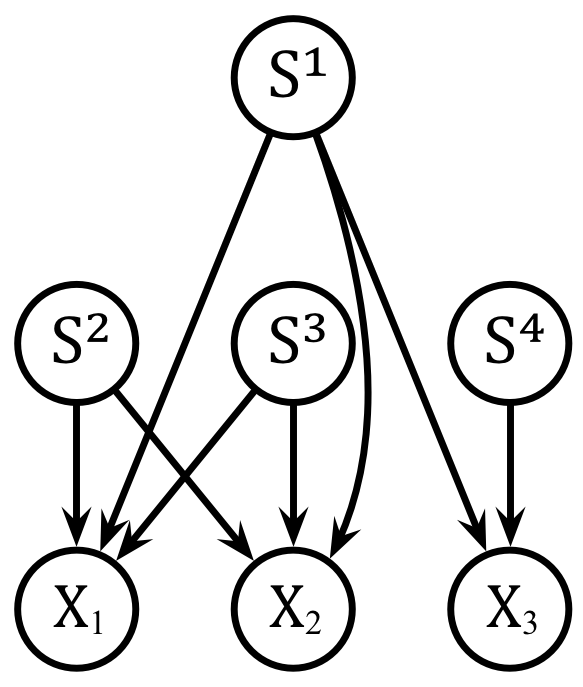
\includegraphics[width=0.25\textwidth]{figures/bn_poupart.png}
		\caption{BN generated by applying Algorithm \ref{alg:poupart} on the normalized SPN in Figure \ref{fig:norm_spn}.}
	\label{fig:bn_poupart}
    \end{center}
\end{figure}

\begin{algorithm}[!ht]
    \caption{\cite{zhao2015relationship} Build BN Structure.}
    \label{alg:poupart}
    \begin{algorithmic}[1]
%        \Procedure{CircuitPropagation}{${\cal AC}$,$\upsilon()$,$d()$}
        \item[\textbf{Input:} normal SPN $\cal S$]
%        \Statex{Normal SPN $\cal S$}
        \item[\textbf{Output:} BN ${\cal B} = ({\cal B}_V, {\cal B}_E)$]
%		\item[\textbf{Main:}]
		\State $R \leftarrow$ root of ${\cal S}$
		\If{$R$ is a terminal node over variable $X$}
			\State Create an observable variable $X$
			\State ${\cal B}_V \leftarrow {\cal B}_V \cup X$
		\Else
			\For{each child $R_i$ of $R$}
				\If{BN has not been built for ${\cal S}_{R_i}$}
					\State Recursively build BN Structure for ${\cal S}_{R_i}$
				\EndIf
			\EndFor
			\If{$R$ is a sum node}
				\State Create a hidden variable $H_R$ associated with $R$
				\State ${\cal B}_V \leftarrow {\cal B}_V \cup \{H_R\}$
				\For{each observable variable $X \in {\cal S}_R$}
					\State ${\cal B}_E \leftarrow {\cal B}_E \cup \{(H_R,X)\}$
				\EndFor
			\EndIf
		\EndIf		
%    \EndProcedure
    \end{algorithmic}
\end{algorithm}

Comment

\subsection{Peharz}

SPN $\rightarrow$ Augumented SPN $\rightarrow$ Peharz BN

Definition

\cite{peharz2013greedy} can define a BN representing an augmented SPN as follows:
for each sum node $S$, connect latent variable $Z_p$ in $An(S)$, connect $Z$ as parent of its associate latent variable $Z_S$, and for all random variable in $scope(S)$ as children of $Z_S$.

\begin{figure}[h]
    \begin{center}
		\includegraphics[width=0.85\textwidth]{figures/aug_SPN.png}
		\caption{Augmentation of SPN in Figure \ref{fig:spn} with latent variables.}
	\label{fig:aug_spn}
    \end{center}
\end{figure}

\begin{figure}[h]
    \begin{center}
		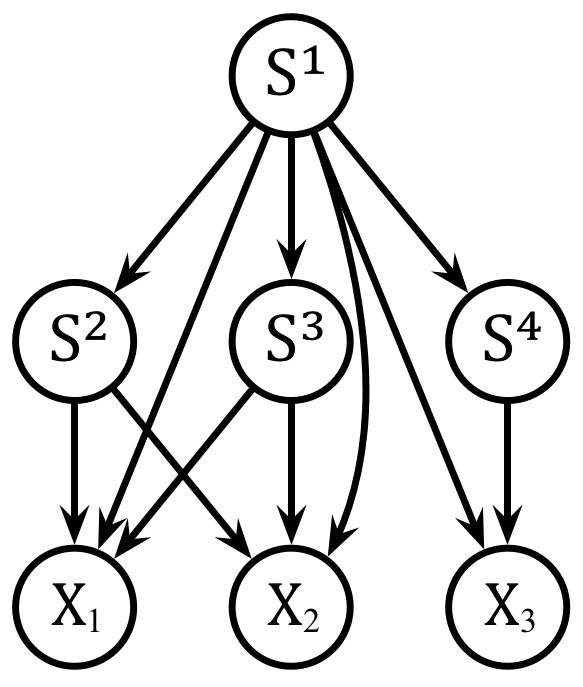
\includegraphics[width=0.25\textwidth]{figures/bn_peharz.png}
		\caption{BN generated by latent variable interpretation given by \cite{peharz2015theoretical} on the augmented SPN in Figure \ref{fig:aug_spn}.}
		\label{fig:bn_poupart}
    \end{center}
\end{figure}

Comment